\documentclass[12pt]{article}
\usepackage[left=1cm, right=1cm, top=2cm,bottom=1.5cm]{geometry} 

\usepackage[parfill]{parskip}
\usepackage[utf8]{inputenc}
\usepackage[T2A]{fontenc}
\usepackage[russian]{babel}
\usepackage{enumitem}
\usepackage[normalem]{ulem}
\usepackage{amsfonts, amsmath, amsthm, amssymb, mathtools}
\usepackage{tabularx}
\usepackage{hhline}

\usepackage{accents}
\usepackage{fancyhdr}
\pagestyle{fancy}
\renewcommand{\headrulewidth}{1.5pt}
\renewcommand{\footrulewidth}{1pt}

\usepackage{graphicx}
\usepackage[figurename=Рис.]{caption}
\usepackage{subcaption}
\usepackage{float}

%%Наименование папки откуда забирать изображения
\graphicspath{ {./images/} }

%%Изменение формата для ввода доказательства
\renewcommand{\proofname}{$\square$  \nopunct}
\renewcommand\qedsymbol{$\blacksquare$}

%%Изменение отступа на таблицах
\addto\captionsrussian{%
	\renewcommand{\proofname}{$\square$ \nopunct}%
}
%% Римские цифры
\newcommand{\RN}[1]{%
	\textup{\uppercase\expandafter{\romannumeral#1}}%
}

%% Для удобства записи
\newcommand{\MR}{\mathbb{R}}
\newcommand{\MQ}{\mathbb{Q}}
\newcommand{\MN}{\mathbb{N}}
\newcommand{\MI}{\mathrm{I}}
\newcommand{\MJ}{\mathrm{J}}
\newcommand{\MH}{\mathrm{H}}
\newcommand{\MT}{\mathrm{T}}
\newcommand{\MU}{\mathcal{U}}
\newcommand{\MV}{\mathcal{V}}
\newcommand{\VN}{\varnothing}
\newcommand{\VE}{\varepsilon}

\theoremstyle{definition}
\newtheorem{defn}{Опр:}
\newtheorem{rem}{Rm:}
\newtheorem{prop}{Утв.}
\newtheorem{exrc}{Упр.}
\newtheorem{lemma}{Лемма}
\newtheorem{theorem}{Теорема}
\newtheorem{corollary}{Следствие}

\newenvironment{cusdefn}[1]
{\renewcommand\thedefn{#1}\defn}
{\enddefn}

\DeclareRobustCommand{\divby}{%
	\mathrel{\text{\vbox{\baselineskip.65ex\lineskiplimit0pt\hbox{.}\hbox{.}\hbox{.}}}}%
}
%Короткий минус
\DeclareMathSymbol{\SMN}{\mathbin}{AMSa}{"39}
%Длинная шапка
\newcommand{\overbar}[1]{\mkern 1.5mu\overline{\mkern-1.5mu#1\mkern-1.5mu}\mkern 1.5mu}
%Функция знака
\DeclareMathOperator{\sgn}{sgn}

%Обозначение константы
\DeclareMathOperator{\const}{\text{const}}

%Интеграл в большом формате
\DeclareMathOperator{\dint}{\displaystyle\int}

\newcommand{\smallerrel}[1]{\mathrel{\mathpalette\smallerrelaux{#1}}}
\newcommand{\smallerrelaux}[2]{\raisebox{.1ex}{\scalebox{.75}{$#1#2$}}}

\newcommand{\smallin}{\smallerrel{\in}}
\newcommand{\smallnotin}{\smallerrel{\notin}}

\newcommand*{\medcap}{\mathbin{\scalebox{1.25}{\ensuremath{\cap}}}}%
\newcommand*{\medcup}{\mathbin{\scalebox{1.25}{\ensuremath{\cup}}}}%

\makeatletter
\newcommand{\vast}{\bBigg@{3.5}}
\newcommand{\Vast}{\bBigg@{5}}
\makeatother

%Скалярное произведение
\DeclarePairedDelimiterX{\inner}[2]{\langle}{\rangle}{#1, #2}

%Подпись символов снизу
\newcommand{\ubar}[1]{\underaccent{\bar}{#1}}

\begin{document}
\lhead{Математический анализ - \RN{2}}
\chead{Шапошников С.В.}
\rhead{Лекция - 17}
\section*{Теорема о неявной функции}
\subsection*{Замечания к теореме о неявной функции}
\begin{rem}
	Пусть есть функция $F(x_1, \dotsc, x_n, y) \colon \MR_x^n \times \MR_y \to \MR$. Пусть для неё выполняются условия теоремы о неявной функции и $\exists \, y =f(x)$, тогда теорема утверждает следующее: 
	$$
		y = f(x) \Leftrightarrow F(x,y) = 0
	$$
	где $f(x)$ непрерывно дифференцируема. Как находить производные функции $f(x)$? 
	
	Чтобы найти производную функции $f \colon \MU(x_0) \to \MV(y_0)$ рассмотрим следующее выражение:
	$$
		\forall x \in \MU(x_0), \, F(x, f(x)) = 0
	$$
	это дифференцируемая функция как композиция двух дифференцируемых функций (одна по условию, другая по теореме). Вычислим частную производную у этого выражения:
	$$
		0 = \dfrac{\partial}{\partial x_k} F(x,f(x)) = \dfrac{\partial F}{\partial x_k}(x, f(x)) + \dfrac{\partial F}{\partial y}(x,f(x)){\cdot}\dfrac{\partial f}{\partial x_k}(x)
	$$
	таким образом, мы можем выразить производную функции $f$ по переменной $x_k$:
	$$
		\dfrac{\partial f}{\partial x_k}(x) = - \displaystyle\dfrac{\dfrac{\partial F}{\partial x_k}(x,f(x))}{\dfrac{\partial F}{\partial y}(x,f(x))}
	$$
\end{rem}
\begin{rem}
	По теореме о неявной функции найдутся окрестности $\MU(x_0), \, \MV(y_0)$ и непрерывно дифференцируемая функция $f \colon \MU \to \MV$ такие, что в окрестности $\MU \times \MV$ верно $y =f(x) \Leftrightarrow F(x,y) = 0$.
	
	Предположим, что есть другая функция $f_1 \colon \MU \to \MV$ такая, что $y = f_1(x) \Leftrightarrow F(x,y) = 0 \Rightarrow f_1(x) = f(x)$. Почему так? Пусть $x \in \MU(x_0)$, рассмотрим $y = f(x) \Rightarrow F(x,y) = 0 \Rightarrow y = f_1(x) \Rightarrow f_1(x) = f(x)$. Важно отметить, что другая функция определена в тех же окрестностях, причем она может быть любой.
	
	Теорема о неявной функции описывает множество $F = 0$. Пусть мы выбрали в нём точку $(x_0, y_0)$ и мы утверждаем, что существует прямоугольник в котором это множество есть график функции, причем эта функция определена однозначно. Данное утверждение верно только локально, но не верно глобально. Это неправда что такая функция одна, если не требовать, чтобы $y$ лежал в $\MV(y_0)$.
	
	Например, рассмотрим окружность: $x^2 + y^2 =1$. На ней есть прямоугольник $\MU \times \MV$, где уравнение равносильно $y = \sqrt{1 - x^2}$. Но если будем говорить только про $\MU$, то таких функций может быть много.
	\begin{figure}[H]
		\centering
		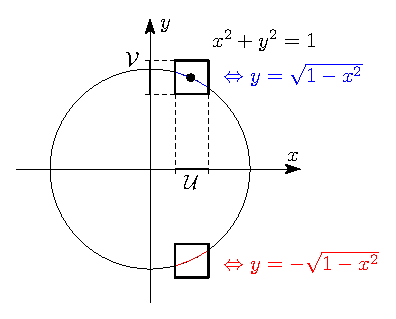
\includegraphics[width=0.35\textwidth]{17_1.eps}
		\caption{Неоднозначность функции $f$ на $\MU$.}
		\label{17_1}
	\end{figure}
\end{rem}

\newpage
\section*{Производные высоких порядков}
\begin{defn}
	Пусть $f\colon \MR^n \to \MR$. Предположим, что в окрестности точки $a$ существует $\tfrac{\partial f}{\partial x_k}$. Если функция $x \mapsto \tfrac{\partial f}{\partial x_k}(x)$ имеет частную производную по $x_m$ в точке $a$, то выражение 
	$$
		\dfrac{\partial}{\partial x_m} \bigg(\dfrac{\partial f}{\partial x_k}(x)\bigg)\bigg|_{x= a}
	$$ 
	называют \uwave{частной производной второго порядка} по $x_k, x_m$ в точке $a$ и обозначают:
	$$
		\dfrac{\partial^2 f}{\partial x_m \partial x_k}(a)
	$$
\end{defn}
Аналогичным образом определяются производные любого порядка:
$$
	\dfrac{\partial^l f}{\partial x_{i_1}\partial x_{i_2}\dotsc \partial x_{i_l}}(a) = \dfrac{\partial}{\partial x_{i_1}}\bigg(\dfrac{\partial}{\partial x_{i_2}}\bigg(\dotsc \bigg(\dfrac{\partial f}{\partial x_{i_l}}(x)\bigg)\dotsc\bigg) \bigg)\bigg|_{x=a}
$$
\begin{defn}
	Пусть $f\colon \MR^n \to \MR$. Предположим, что в окрестности точки $a$ существует $\tfrac{\partial^{m-1} f}{\partial x_{i_1}\dotsc \partial x_{i_{m-1}}}$. Если функция 
	$$
		x \mapsto \dfrac{\partial^{m-1} f}{\partial x_{i_1}\dotsc \partial x_{i_{m-1}}}(x)
	$$ 
	имеет частную производную по $x_{i_m}$ в точке $a$, то выражение 
	$$ 
		\dfrac{\partial}{\partial x_{i_1}}\bigg(\dfrac{\partial}{\partial x_{i_2}}\bigg(\dotsc \bigg(\dfrac{\partial f}{\partial x_{i_m}}(x)\bigg)\dotsc\bigg) \bigg)\bigg|_{x = a}
	$$
	называют \uwave{частной производной $m$-го порядка} по $x_{i_1},\dotsc, x_{i_m}$ в точке $a$ и обозначают:
	$$
		\dfrac{\partial^m f}{\partial x_{i_1}\partial x_{i_2}\dotsc \partial x_{i_m}}(a)
	$$
\end{defn}
Зависит ли производная от порядка переменных $i_1, \dotsc, i_l$? Например, для функции $xy\tfrac{x^2 - y^2}{x^2 + y^2}$. В общем случае - зависит, но чаще всего нет и на это есть две теоремы.
\begin{theorem}(Юнг)
	Пусть $f\colon \MR^2 \to \MR$ и в окрестности точки $a$ существуют $\tfrac{\partial f}{\partial x}$ и $\tfrac{\partial f}{\partial y}$. Если эти производные $\tfrac{\partial f}{\partial x}$ и $\tfrac{\partial f}{\partial y}$ как функции дифференцируемы в точке $a$, то:
	$$
		\dfrac{\partial^2 f}{\partial x \partial y}(a) = \dfrac{\partial^2 f}{\partial y \partial x}(a)
	$$
\end{theorem}
\begin{rem}
	Частные производные дифференцируемы в точке $a \Rightarrow$ они непрерывны в точке $a \Rightarrow$ эта функция в точке $a$ - дифференцируема (по теореме о достаточном условии дифференцируемости).
\end{rem}
\begin{proof}
	Удобно считать что $a = (0,0)$. Составим следующее выражение (второе разностное соотношение): 
	$$
		\Delta(t) = f(t,t) - f(t,0) - f(0,t) + f(0,0)
	$$
	Оно имеет такой вид из следующего соображения:
	$$
		\dfrac{\partial^2 f}{\partial x \partial y} \approx \dfrac{\tfrac{\partial f}{\partial y}(x + \Delta x) - \tfrac{\partial f}{\partial y}(x)}{\Delta x} \approx \dfrac{\big(f(x + \Delta x, y + \Delta y) - f(x + \Delta x, y)\big) - \big(f(x, y + \Delta y) - f(x, y)\big)}{\Delta x \Delta y}
	$$
	подставив в него значения $x = y =0, \, \Delta x = \Delta y = t$ получим:
	$$
		\dfrac{\partial^2 f}{\partial x \partial y} \approx \dfrac{f(t,t) - f(t,0) - f(0,t) + f(0,0)}{t^2} = \dfrac{\Delta(t)}{t^2}
	$$
	Если заменить $x$ и $y$ местами в смешанной производной, то получим такое же выражение, поскольку оно симметрично по $x$ и $y$ (берем сначала разность по $x$, а затем по $y \Leftrightarrow$ сначала взять разность по $y$, а затем по $x$). Этому выражению приближенно равны смешанные производные, тогда отсюда должно бы следовать что они тоже симметричны по $x$ и $y$. 
	
	Проблема состоит в том, чтобы показать что при стремлении $\Delta x, \, \Delta y$ к нулю, в пределе мы действительно получим равенство вместо приближенного равенства. Это затрудняется тем, что каждая из разностей ведет себя по-разному в зависимости от значения $\Delta y$.
	
	Перепишем выражение $\Delta(t)$ в другом виде и воспользуемся теоремой Лагранжа:
	$$
		\Delta(t) = \Big(f(x,t) - f(x,0)\Big)\Big|_0^t = \varphi(x)\Big|_0^t =  \varphi(t) - \varphi(0) = \varphi^\prime(c){\cdot}t = \bigg(\dfrac{\partial f}{\partial x}(c,t) - \dfrac{\partial f}{\partial x}(c,0)\bigg){\cdot}t, \, c \in (0,t)
	$$
	Мы знаем, что $\dfrac{\partial f}{\partial x}$ дифференцируем в $(0,0)$, по определению это означает:
	$$
		\dfrac{\partial f}{\partial x}(b_1,b_2) - \dfrac{\partial f}{\partial x}(0,0) = \dfrac{\partial}{\partial x}\bigg( \dfrac{\partial f}{\partial x}\bigg)(0,0){\cdot}b_1 + \dfrac{\partial}{\partial y}\bigg( \dfrac{\partial f}{\partial x}\bigg)(0,0){\cdot}b_2 + \overline{o}\Big(\sqrt{b_1^2 + b_2^2}\Big)
	$$
	где $\overline{o}$ стремится к нулю, когда $b_1, \, b_2$ стремятся к нулю. Применим это разложение к $\dfrac{\partial f}{\partial x}$ в точке $(c,t)$:
	$$
		\dfrac{\partial f}{\partial x}(c,t) = \dfrac{\partial f}{\partial x}(0,0) + \dfrac{\partial^2 f}{\partial x^2}(0,0){\cdot}c + \dfrac{\partial^2 f}{\partial y \partial x}(0,0){\cdot}t + \overline{o}\Big(\sqrt{c^2 + t^2}\Big)
	$$
	Аналогично применим разложение к $\dfrac{\partial f}{\partial x}$ в точке $(c,0)$:
	$$
		\dfrac{\partial f}{\partial x}(c,0) = \dfrac{\partial f}{\partial x}(0,0) + \dfrac{\partial^2 f}{\partial x^2}(0,0){\cdot}c + \dfrac{\partial^2 f}{\partial y \partial x}(0,0){\cdot}0 + \overline{o}\Big(\sqrt{c^2 + 0}\Big)
	$$
	Подставим оба выражения в записанную ранее разность $\Delta(t)$:
	$$
		\Delta(t) = \bigg(\dfrac{\partial^2 f}{\partial y \partial x}(0,0){\cdot}t + \overline{o}\Big(\sqrt{c^2 + t^2}\Big) - \overline{o}\big(|c|\big)\bigg){\cdot}t = \dfrac{\partial^2 f}{\partial y \partial x}(0,0){\cdot}t^2 + \overline{o}\Big(\sqrt{c^2 + t^2}\Big){\cdot}t - \overline{o}\big(|c|{\cdot}t\big)
	$$
	Заметим, что поскольку $0 < c < t$, то из $t \to 0 \Rightarrow c \to 0$, также отметим, что $\lim\limits_{t \to 0}\overline{o}(1) = 0$. Тогда:
	$$
		\dfrac{|c|{\cdot}|t|}{t^2} = \dfrac{|c|}{|t|} < 1 \Rightarrow 
		0 \leq \overline{o}\bigg(\dfrac{|c|{\cdot}|t|}{t^2}\bigg) = \overline{o}\bigg(1{\cdot} \dfrac{|c|}{|t|}\bigg) = \overline{o}(1){\cdot} \dfrac{|c|}{|t|} < \overline{o}(1) \to 0 \Rightarrow 
		\lim\limits_{t\to 0} \overline{o}\bigg(\dfrac{|c|{\cdot}|t|}{t^2}\bigg) = 0
	$$
	$$
		\dfrac{\sqrt{c^2 + t^2}{\cdot}|t|}{t^2} = \sqrt{1 + \dfrac{c^2}{t^2}}  < \sqrt{2} \Rightarrow 
		0 \leq \overline{o}\bigg(\dfrac{\sqrt{c^2 + t^2}{\cdot}|t|}{t^2}\bigg) < \overline{o}(1){\cdot}\sqrt{2} \to 0 \Rightarrow 
		\lim\limits_{t\to 0}\overline{o}\bigg(\dfrac{\sqrt{c^2 + t^2}{\cdot}|t|}{t^2}\bigg) = 0
	$$
	Следовательно, рассмотрим, куда стремится отношение $\dfrac{\Delta(t)}{t^2}$ при $t \to 0$:
	$$
		\lim\limits_{t \to 0} \dfrac{\Delta(t)}{t^2}  = \dfrac{\partial^2 f}{\partial y \partial x}(0,0) + \lim\limits_{t\to 0}\overline{o}\bigg(\dfrac{\sqrt{c^2 + t^2}{\cdot}|t|}{t^2}\bigg) - \lim\limits_{t\to 0} \overline{o}\bigg(\dfrac{|c|{\cdot}|t|}{t^2}\bigg) = \dfrac{\partial^2 f}{\partial y \partial x}(0,0)
	$$
	Аналогичным образом, поменяв местами $x$ и $y$, проделываем те же шаги, выражение $\Delta(t)$ от этого не поменяется и следовательно мы получим:
	$$
		\lim\limits_{t \to 0} \dfrac{\Delta(t)}{t^2} = \dfrac{\partial^2 f}{\partial x \partial y}(0,0)
	$$
	Вспоминая что предел у нас единственный, мы приходим к выводу:
	$$
		\lim\limits_{t \to 0} \dfrac{\Delta(t)}{t^2} = \dfrac{\partial^2 f}{\partial x \partial y}(0,0) = \dfrac{\partial^2 f}{\partial y \partial x}(0,0)
	$$
\end{proof}
\begin{theorem}(Шварц)
	Пусть $f\colon \MR^2 \to \MR$ и в окрестности точки $a$ существуют $\tfrac{\partial^2 f}{\partial x\partial y}$ и $\tfrac{\partial^2 f}{\partial y \partial x}$. Если эти производные непрерывны в точке $a$, то они в этой точке совпадают:
	$$
		\dfrac{\partial^2 f}{\partial x \partial y}(a) = \dfrac{\partial^2 f}{\partial y \partial x}(a)
	$$
\end{theorem}
\begin{rem}
	Теоремы Шварца и Юнга отличаются друг от дргуа: 
	\begin{enumerate}[label ={(\arabic*)}]
		\item В теореме Юнга предполагается, что частные производные дифференцируемы$ \Leftrightarrow \, \exists$ как вторые производные, так и смешанные производные. Заметим что, если функция дифференцируема, то её производная не обязана быть непрерывной;
		\item В теореме Шварца не утверждается существование второй производной, при этом требуется непрерывность смешанных производных;
	\end{enumerate}
\end{rem}
\begin{proof}
	Доказательство похоже на доказательство теоремы Юнга. Удобно считать что $a = (0,0)$. Составим функцию $\Delta(t,s)$ вида: 
	$$
		\Delta(t,s) = f(t,s) - f(t,0) - f(0,s) + f(0,0)
	$$
	Она имеет такой вид из следующего соображения:
	$$
		\dfrac{\partial^2 f}{\partial x \partial y} \approx \dfrac{\tfrac{\partial f}{\partial y}(x + \Delta x) - \tfrac{\partial f}{\partial y}(x)}{\Delta x} \approx \dfrac{\big(f(x + \Delta x, y + \Delta y) - f(x + \Delta x, y)\big) - \big(f(x, y + \Delta y) - f(x, y)\big)}{\Delta x \Delta y}
	$$
	подставив в него значения $x = y =0, \, \Delta x = t, \, \Delta y = s$ получим:
	$$
		\dfrac{\partial^2 f}{\partial x \partial y} \approx \dfrac{f(t,s) - f(t,0) - f(0,s) + f(0,0)}{ts} = \dfrac{\Delta(t,s)}{ts}
	$$
	Если заменить $x$ и $y$ местами в смешанной производной, то получим такое же выражение, поскольку оно симметрично по $x$ и $y$ (берем сначала разность по $x$, а затем по $y \Leftrightarrow$ сначала взять разность по $y$, а затем по $x$). Этому выражению приближенно равны смешанные производные, тогда отсюда должно бы следовать что они тоже симметричны по $x$ и $y$. 
	
	Проблема состоит в том, чтобы показать что при стремлении $\Delta x, \, \Delta y$ к нулю, в пределе мы действительно получим равенство вместо приближенного равенства. 
	
	Перепишем выражение $\Delta(t,s)$ в другом виде и воспользуемся теоремой Лагранжа:
	$$
		\Delta(t,s) = \Big(f(x,s) - f(x,0)\Big)\Big|_0^t = \varphi(x)\Big|_0^t =  \varphi(t) - \varphi(0) = \varphi^\prime(c){\cdot}t = \bigg(\dfrac{\partial f}{\partial x}(c,s) - \dfrac{\partial f}{\partial x}(c,0)\bigg){\cdot}t, \, c \in (0,t)
	$$
	Рассмотрим следующую функцию $\psi(u) = \tfrac{\partial f}{\partial x}(c,u)$, тогда выражение выше перепишется следующим образом:
	$$
		\varphi^\prime(c) = \dfrac{\partial f}{\partial x}(c,s) - \dfrac{\partial f}{\partial x}(c,0) = \psi(s) - \psi(0)
	$$
	Снова воспользуемся теоремой Лагранжа и получим следующий результат:
	$$
		\psi(s) - \psi(0) = \psi^\prime(d){\cdot}s = \dfrac{\partial}{\partial y}\bigg(\dfrac{\partial f}{\partial x}(c,u)\bigg)\bigg|_{u = d} = \dfrac{\partial^2 f}{\partial y\partial x}(c,d), \, 0 < c < t, \, 0 < d < s
	$$
	Таким образом мы получили, что наша функция $\Delta(t,s)$ выражается в виде смешанной производной:
	$$
		\Delta(t,s) = \dfrac{\partial^2 f}{\partial y\partial x}(c,d), \, 0 < c < t, \, 0 < d < s
	$$
	Сделаем группировку в другом порядке и получим аналогичный результат:
	$$
		\Delta(t,s) = \dfrac{\partial^2 f}{\partial x\partial y}(\widetilde{c},\widetilde{d}), \, 0 < \widetilde{c} < t, \, 0 < \widetilde{d} < s
	$$
	Заметим, что из теореме Лагранжа верно следующее: 
	$$
		t \to 0 \Rightarrow c \to 0 \wedge \widetilde{c} \to 0 
	$$
	$$
		s \to 0 \Rightarrow d \to 0 \wedge \widetilde{d} \to 0
	$$ 
	Тогда в силу непрерывности смешанных производных мы получим:
	$$
		\lim\limits_{t \to 0}\lim\limits_{s \to 0}\Delta(t,s) = \lim\limits_{t \to 0}\lim\limits_{s \to 0}\dfrac{\partial^2 f}{\partial y\partial x}(c,d) = \dfrac{\partial^2 f}{\partial y\partial x}(0,0) 
	$$
	$$
		\lim\limits_{t \to 0}\lim\limits_{s \to 0}\Delta(t,s)= \lim\limits_{t \to 0}\lim\limits_{s \to 0}\dfrac{\partial^2 f}{\partial x\partial y}(\widetilde{c},\widetilde{d}) = \dfrac{\partial^2 f}{\partial x\partial y}(0,0)
	$$
	В силу единственности предела мы получим, что:
	$$
		\dfrac{\partial^2 f}{\partial y\partial x}(0,0)  = \dfrac{\partial^2 f}{\partial x\partial y}(0,0)
	$$
\end{proof}

\textbf{Пример}: Рассмотрим функцию $f(x,y) = g(x) + h(y)$, где функции $g, \, h$ - один раз дифференцируемы (функции одной  переменной). Найдем её частные производные:
$$
	\dfrac{\partial f}{\partial x} = g^\prime(x), \, \dfrac{\partial f}{\partial y} = h^\prime(y)
$$
Эти функции не обязаны быть непрерывными, теорема Юнга сюда неприменима. Рассмотрим смешанные производные:
$$
	\dfrac{\partial^2 f}{\partial y\partial x} = 0, \, \dfrac{\partial^2 f}{\partial x\partial y} = 0
$$
Таким образом теорема Шварца в этом примере выполнена, а теорема Юнга - нет.

\begin{defn}
	Пусть $f\colon \MR^n \to \MR$ дифференцируема в окрестности точки $a$ \big(тогда в этой окрестности $\exists$ все частные производные $\tfrac{\partial f}{\partial x_k}$\big). Если все функции $x \mapsto \tfrac{\partial f}{\partial x_k}$ дифференцируемы в точке $a$ ($\forall k$), то говорят, что $f$ \uwave{дважды дифференцируема в точке} $a$.
\end{defn}

\begin{defn}
	Пусть уже определено, что значит $f$ $m$-раз дифференцируема. Если $f$ $m$-раз дифференцируема в окрестности точки $a$ и все её частные производные $m$-го порядка дифференцируемы в точке $a$, то говорят, что $f$ $(m+1)$-\uwave{раз дифференцируема в точке} $a$.
\end{defn}

\begin{corollary}
	Если $f$ $m$-раз дифференцируема в точке $a$, то значение выражения $\tfrac{\partial^m f}{\partial x_{i_1} \dotsc \partial x_{i_m}}(a)$ не зависит от порядка переменных (индексы среди $i_1, \dotsc, i_m$ могут повторяться).
\end{corollary}
\begin{proof}
	Поскольку функция $f$ дифференцируема $m$-раз $\Rightarrow$ она дифференцируема два раза $\Rightarrow$ по теореме Юнга будет верно:
	$$
		\dotsc \bigg(\dfrac{\partial^2 }{\partial x_{i_k} \partial x_{i_{k+1}}} \bigg(\dotsc\bigg) \bigg)\dotsc  = \dotsc \bigg(\dfrac{\partial^2 }{\partial x_{i_{k+1}} \partial x_{i_k} } \bigg(\dotsc\bigg) \bigg)\dotsc
	$$
	Таким образом, если умеем перестовлять два соседних элемента, то можем переставить любые два элемента.
	
	Также можно доказать по индукции: пусть мы умеем делать перестановку любых элементов в $\tfrac{\partial^{m-1} f}{\partial x_{i_2} \dotsc \partial x_{i_m} }$. Тогда в $m$-ой производной:
	$$
		\dfrac{\partial^m f}{\partial x_{i_1} \partial x_{i_2} \dotsc \partial x_{i_m}} = \dfrac{\partial }{\partial x_{i_1}}\bigg(\dfrac{\partial^{m-1} f}{\partial x_{i_2} \dotsc \partial x_{i_m} } \bigg)
	$$
	применяем теорему Юнга и получаем требуемый результат.
\end{proof}

\newpage
\section*{Дифференциалы высоких порядков}
\subsection*{Второй дифференциал}
Пусть $f \colon \MR^n \to \MR$ дважды дифференцируема в точке $a$. То есть $f$ один раз дифференцируема в окрестности точки $a$ и все функции $x \mapsto \tfrac{\partial f}{\partial x_k}$ дифференцируемы в точке $a$. Рассмотрим у этой функции первый дифференциал:
$$
	df(x,h) = \dfrac{\partial f}{\partial x_1}(x){\cdot}h_1 + \dotsc + \dfrac{\partial f}{\partial x_n}(x){\cdot}h_n
$$
Зафиксируем $h$ и будем смотреть на функцию $df(x,h)$ как на функцию от $x$. Поскольку дано, что $\tfrac{\partial f}{\partial x_k}$ это дифференцируемые в точке $a$ функции, то $x \mapsto df(x,h)$ дифференцируема в точке $a \Rightarrow$ можно найти её дифференциал в точке $a$ от вектора $v$:
$$
	d\big(d(f,h)\big)(a,v) = \dfrac{\partial}{\partial x_1}\big(df(x,h)\big)(a){\cdot}v_1 + \dotsc + \dfrac{\partial}{\partial x_n}\big(df(x,h)\big)(a){\cdot}v_n = 
$$
$$
	= \dfrac{\partial^2 f}{\partial x_1^2}(a){\cdot}h_1{\cdot}v_1 + \dotsc + \dfrac{\partial^2 f}{\partial x_1 \partial x_n}(a){\cdot}h_n{\cdot}v_1 + \dotsc + \dfrac{\partial^2 f}{\partial x_n \partial x_1}(a){\cdot}h_1{\cdot}v_n + \dotsc + \dfrac{\partial^2 f}{\partial x_n^2}(a){\cdot}h_n{\cdot}v_n =
$$
$$
	= \displaystyle \sum\limits_{i,j}\dfrac{\partial^2 f}{\partial x_i \partial x_j}(a){\cdot}h_j{\cdot}v_i = B(h,v)
$$
Из формулы выше очевидно, что это выражение линейно по $h$ и по $v$, то есть $B(h,v)$ - билинейная форма. По теореме Юнга: $\tfrac{\partial^2 f}{\partial x_i \partial x_j}(a) = \tfrac{\partial^2 f}{\partial x_j \partial x_i}(a)\Rightarrow$ можно поменять местами индексы или, что то же самое, поменять местами $h$ и $v$. Тогда:
$$
	B(h,v) =\displaystyle \sum\limits_{i,j}\dfrac{\partial^2 f}{\partial x_i \partial x_j}(a){\cdot}h_j{\cdot}v_i = \displaystyle \sum\limits_{i,j}\dfrac{\partial^2 f}{\partial x_j \partial x_i}(a){\cdot}v_i{\cdot}h_j = B(v,h)
$$
Таким образом, $B(h,v)$ - симметричная билинейная форма. Из линейной алгебры мы знаем, что такая форма однозначно задается квадратичной, то есть $B(h,h) = Q(h) \Rightarrow$ вся информация про эту симметричную билинейную форму содержится в квадратичной форме.
\begin{defn}
	\uwave{Второй дифференциал} это $d^2f(a,h) = B(h,h) = d\big(df(x,h)\big)(a,h) = \displaystyle \sum\limits_{i,j}\dfrac{\partial^2 f}{\partial x_i \partial x_j}(a){\cdot}h_j{\cdot}h_i$.
\end{defn} 
\begin{rem}
	Мы обсуждали, что есть функции $dx_i(h) = h_i$, если мы их используем, то $d^2f(a,h)$ запишется следующим образом:
	$$
		d^2f(a,h) = \displaystyle \sum\limits_{i,j}\dfrac{\partial^2 f}{\partial x_i \partial x_j}(a){\cdot}\big(dx_j(a,h)\big){\cdot}\big(dx_i(a,h)\big) \Leftrightarrow d^2f = \displaystyle \sum\limits_{i,j}\dfrac{\partial^2 f}{\partial x_i \partial x_j}{\cdot}(dx_j){\cdot}(dx_i)
	$$
	Отсюда необходимо иметь в виду, что $dx^2 = (dx)^2$.
\end{rem}
\begin{rem}
	При решении задач обычно первый дифференциал записывается следующим образом:
	$$
		df = \dfrac{\partial f}{\partial x_1}(x)dx_1 + \dotsc + \dfrac{\partial f}{\partial x_n}(x)dx_n
	$$
	Затем, чтобы взять второй дифференциал, мы вычисляем дифференциалы каждой из функций $\tfrac{\partial f}{\partial x_i}$, считая при этом что $dx_i$ - константы. Это ровно то, что мы проделали выше зафиксировав $h$ и считая дифференциал. Но при дифференцировании $\tfrac{\partial f}{\partial x_i}$ мы используем те же самые $dx_1, \dotsc, dx_n$ и получаем: 
	$$
		d^2f = \displaystyle \sum\limits_{i,j}\dfrac{\partial^2 f}{\partial x_i \partial x_j}{\cdot}(dx_j){\cdot}(dx_i)
	$$
	Это происходит по причине перехода от билинейной формы к квадратичной и тем самым мы выписываем не значения на векторе $h$ и затем на векторе $v$, а значения на одном и том же векторе $h$.
\end{rem}
\begin{rem}
	При замене переменных, в выражениях содержащих вторые производные, необходимо учитывать, что нельзя вычислять второй дифференциал композиции просто подставляя $dx_i, \, dx_j$ поскольку не выполняется инвариантность и приходится дифференцировать еще раз функции, которые заменяют переменные.
\end{rem}
\subsection*{Дифференциалы $m$-го порядка}
\begin{defn}
	Пусть $f\colon \MR^n \to \MR$ $m$-раз дифференцируема в точке $a$, тогда выражение:
	$$
		d^mf(a,h) = \displaystyle \sum\limits_{i_1 \dotsc i_m}\dfrac{\partial^m f}{\partial x_{i_1} \dotsc \partial x_{i_m}}(a){\cdot}h_{i_1}{\cdot}\dotsc{\cdot}h_{i_m}, \, i_j \in \{1, \dotsc, n\}, \, \forall j = \overline{1,m}
	$$
	называется \uwave{дифференциалом} $m$-\uwave{го порядка} в точке $a$ на векторе $h$.
\end{defn}
\begin{rem}
	Естественное определение дифференциалов $m$-го порядка это полилинейная форма $m$-го порядка. Стоит также отметить, что один из естественных способов получения полилинейных форм это вычисление дифференциалов высокого порядка у отображений. Тогда на месте каждого из $h_{i_j}$ должны стоять координаты своего вектора. Но так устоялось, что у линейного объекта получилась нелинейная структура.
\end{rem}
\begin{prop}
	Пусть $f\colon \MR^n \to \MR$ $(m+1)$-раз дифференцируема в точке $a$, тогда верно следующее равенство:
	$$
		d^{m+1}f(a,h) = d\big(d^mf(x,h)\big)(a,h)
	$$
\end{prop}

\end{document}